\section{\sys Challenges}\label{sec:challenges}
\begin{figure}[t]
% \centering
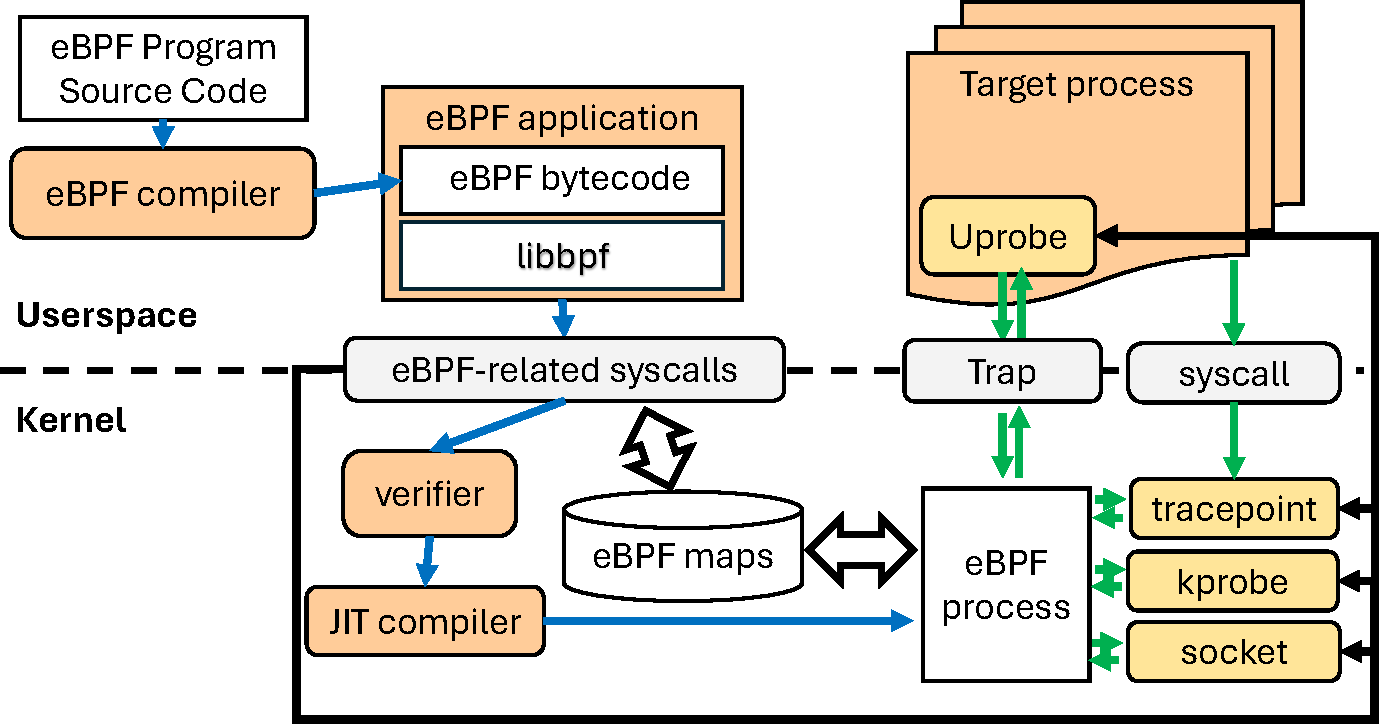
\includegraphics[width=\columnwidth]{img/ebpf-diagram-cropped.pdf}
\caption{eBPF Design Diagram.  Blue arrows indicate the execution flow when a user compiles and loads an eBPF program.  Green arrows indicate the execution flow when an eBPF extension executes.  White arrows with black outline indicate read/write operations to shared memory in the eBPF maps.  Black arrows indicate operations that attach an extension}\label{fig:eBPF-design}
\end{figure}

\sys{} is a comprehensive dynamic, safe, and efficient extension framework.  The system builds on the success of the eBPF ecosystem, which provides many of the design constraints.  However, \sys{} crucially diverges from eBPF in its technique to support extensions to userspace logic.  Namely, rather than execute userspace extension logic in the kernel, which degrades comprehensiveness and efficiency, \sys{} instead creates a new userspace eBPF runtime that uses dynamic binary instrumentation to execute userspace extensions directly in the extended application.

However, execute eBPF extensions in userspace leads to three main challenges: \sys{} must provide a new eBPF runtime, \sys{} must devise a new method for attaching to an arbitrary program, and \sys{} must ensure safety of the user's extensions. 

In the remainder of this section, we first provide background on the current eBPF ecosystem (\cref{sec:challenges:eBPF-background}).  Then, we outline the challenges that arises when extending eBPF execution into userspace (\cref{sec:challenges:details}). 

\subsection{eBPF Background} \label{sec:challenges:eBPF-background}
This section describes the background eBPF knowledge necessary to understand \sys{}.  \Cref{fig:eBPF-design} shows a design diagram of the critical components of the ecosystem and how the components interact.  We discuss the three main phases of interacting with eBPF: Writing an eBPF program, loading an eBPF program, and executing an eBPF program.

\subsubsection{Writing an eBPF program}

A user writes an eBPF program (eBPF Program Source Code).  The user expresses each of the extensions that they wish to add to the system as a separate function. They annotate the hook point for each extension using the syntax \mintinline{c}{SEC("<type>/<name>")} indicating that the function should be executed when the program reaches the hook point \mintinline{c}{name} of probe type \mintinline{c}{type} (\eg \texttt{kprobe}, \texttt{uprobe}, \texttt{uretprobe}, etc.).  The user can leverage a rich set of eBPF helper functions to help with many tasks, including access eBPF maps, read memory, get process information, etc.   The user passes their eBPF program to an eBPF compiler (e.g., \texttt{clang}), which produces eBPF bytecode for the user's extensions. The bytecode consists of the program's extension logic (\ie its functions), maps and their associated hook points as an ELF binary.  

\subsubsection{Loading an eBPF Program}

When the user wishes to execute their extension, they use an existing toolchain (e.g., \texttt{libbpf}) to load the eBPF bytecode.  The toolchain interacts with a number of bpf-related system calls (\eg \mintinline{c}{bpf}, \mintinline{c}{perf_event_open}) to load the extension into the system.  The bpf-related system calls perform three main tasks.  First, some of the eBPF system calls initialize maps for the eBPF program to use. Second, some of the eBPF system calls instrument the actual hook points (e.g., \texttt{uprobe}s, \texttt{kprobe}s, etc.) required by the eBPF program.  The instrumentation adds software breakpoints (\ie \texttt{int 0xcc}) for userspace hook point, and uses trampolines (\ie \texttt{jmp} instructions) for kernel space hook points.  Finally, some of the eBPF system calls validate the eBPF byte code. These calls pass the eBPF bytecode for the user's execution logic to an eBPF verifier.  One important note: the current eBPF ecosystem \emph{does not} verify userspace extensions (\ie those that attach to \texttt{uprobe} and \texttt{uretprobe} hook points).
\yusheng{Might be better to describe as "does not ensure userspace extensions don't break userspace process." because it does verify the uprobe eBPF don't break kernel, like infinity loop or access kernel memory wrong.} \arq{OK. I'm totally confused, then.  I thought that eBPF's uprobes are not able to change the state of the userspace program.  So, I don't understand the distinction that you're drawing here...}

The verifier uses static analysis to ensure that the eBPF bytecode is safe to execute.  Namely, the verifier checks to see if the eBPF bytecode is memory and type safe by checking the type and memory offset of each memory dereference in the bytecode by consulting metadata released with each kernel called the BPF Type Format (BTF).  Next, the verifier ensures that the bytecode terminates by ensuring that all loops have a constant bound, are not recursive.  The verifier validates that there are no hardware exceptions in the eBPF bytecode by checking each instruction.  For example, it checks for divisions by unknown scalars to ensure that an extension cannot cause a divide-by-zero exception.  Lastly, the bytecode verifier ensures that the extension does not leak resources by ensuring that all allocated resources (e.g., ring buffer memory) are released on all possible program paths.

\subsubsection{Executing an eBPF Program}

After the eBPF program is loaded, the system begins executing.  The kernel provides a Just-in-time (JIT) Compiler that takes the verified eBPF bytecode as input and compiles it as necessary to the native architecture of the machine.  The system executes the eBPF bytecode logic each time it reaches a configured hook point.  When the kernel reaches a kernel hook point, the trampoline technique redirects execution to the eBPF extension.  When the userspace application reaches a hook point, the application executes a trap which passes control to the eBPF extension.  This incurs at least two context switches (one to the kernel and one back to userspace), often even more as the system must execute the logic of the instruction located at the software breakpoint, which comes with high overhead.

The eBPF extensions read and modify the system's state.  They use eBPF maps to store execution state across extended hook points, and also to communicate output data to the eBPF application.  The eBPF application can use system calls to read this data, primarily in observability use-cases. 

\subsubsection{DeepFlow Example}
\begin{figure}[t]
\centering
\begin{minted}{c}
struct event {
  u32 saddr_v4;
  u64 goid;
};

BPF_RINGBUF_OUTPUT(rb, 1 << 4);
BPF_HASH(goroutines, u64);

SEC("uprobe/go-server-http:runtime.casgstatus")
int uprobe_runtime_casgstatus(struct pt_regs * ctx) {
  void *gp = ctx->ax;
  u64 goid;
  if (bpf_probe_read_user(&goid, sizeof(goid),
                          gp + GOID_OFFSET) == 0) {
    u64 thread = bpf_get_current_pid_tgid();
    bpf_map_update_elem(&goroutines, &thread, &goid, 0);
  }
  return 0;
}

SEC("kprobe/tcp_v4_connect")
int BPF_KPROBE(tcp_v4_connect, struct sock* sk) {
  u64 thread = bpf_get_current_pid_tgid();
  u64 *goid_p = bpf_map_lookup_elem(&goroutines, &thread);
  if (!goid_p)
    return 0;
  struct event* data;
  data = bpf_ringbuf_reserve(&rb, sizeof(*data), 0);
  if (!data)
    return 0;
  BPF_CORE_READ_INTO(&data.saddr_v4, sk,
    __sk_common.skc_rcv_saddr);
  data->goid = *goid_p;
  bpf_ringbuf_submit(data, 0);
}
\end{minted}
\vspace{-0.5cm}
\caption{A simplified eBPF implementation of DeepFlow. \arq{A few things: First, the definition of goroutoine\_execute\_data is not provided.  Second, I updated the output to be an actual use-cases that someone might do.}} \yusheng{I change it slightly, add data defines and put a read tcp address here to make it correct. This is what people do.} \label{code:example}
\vspace{-0.5cm}
\end{figure}
We outline a small portion of the extensions for DeepFlow (see \cref{sec:motivation:examples}); \cref{code:example} provides the example code.  The program tracks the initial values of low-level socket options (\eg the size of a receive buffer), which are useful for identifying poor performance of socket related operations.  The program attaches logic on the userspace code that schedules \texttt{go-routine}s (\mintinline{c}{runtime.casgstatus}) to track the \texttt{go-routine} \texttt{ID} corresponding to each thread in the program.  It identifies the size of the receive buffer (\texttt{sk\_recvbuf}) of each tcp socket when the socket connects to an endpoint (inside the kernel at function \mintinline{c}{tcp_v4_connect}).  It produces output to a ring buffer of that shows the \texttt{go-routine ID} and the \texttt{sk\_recvbuf} value; the user's eBPF application correlates this output data with request-level tracing to identify if poor request performance is correlated with initial \texttt{sk\_recvbuf} values (this code is not shown).


\subsection{Userspace eBPF Challenges} \label{sec:challenges:details}

\sys{} resolves the efficiency and comprehensively challenges of the current eBPF ecosystem by executing userspace extensions directly in the target process.   The approach is conceptually simple, but it exposes a number of critical challenges: 

% \yusheng{ubpf and rbpf exist}  This includes the kernel's JIT Compiler as well as the many eBPF helper functions that the runtime provides to simplify eBPF program development.  Running an eBPF extension from userspace requires a new userspace runtime and new userspace helpers to fill these gaps.  \yusheng{The actually challenge is that 1. Our goal is provided compatible with existing eBPF toolchains and libraries, but the current eBPF loading process is complex, requires a sets of different syscall, include bpf, perf event open, mmap, epoll, open, close... syscalls, it's typically requires thousands of syscall executions to load and control all the eBPF programs in a eBPF application like deepflow. So the loader is complex and requires 4000 lines. If we don't provide compatibility to the toolchains, then it's impossible to run the large eBPF application like deepflow or even smaller bcc tools like sslsniff.} \yusheng{Another challenge is about eBPF maps. currently the eBPF ecosystem already has userspace jit implement, but not userspace maps implementation, especially we want to have shared maps between userspace and kernel, and shared maps between different userspace. We need to implement a lot of data structures in shared memory. This is critical for the execution of eBPF programs. I have discussed that in ppt.}

\paragraph{A New eBPF runtime for the eBPF Ecosystem} eBPF applications use a vast ecosystem of tooling, including a set of eBPF-related system calls, helper functions, eBPF maps, and eBPF JIT compilers, which must evolve to execute in userspace.  To ensure comprehensiveness, \sys{} must be  compatible this current ecosystem.  This includes seamlessly supporting current eBPF-related systemcalls, providing similar eBPF helper functions for userspace extensions, providing comprehensive eBPF maps, and providing a JIT compiler for executing eBPF code in userspace.  Prior work on userspace eBPF, including ubpf~\cite{ubpf} and rbpf~\cite{rbpf}, support JIT compilers for executign eBPF bytecode in userspace, but do not handle any of the other core issues. 


\paragraph{Attaching to an arbitrary program} The current eBPF ecosystem's logic for attaching to a userpsace program is a simple implementation that replaces program bytes with software breakpoints.  However, attaching to an arbitrary userspace process is significantly more difficult, especially to support extensions on \texttt{syscall tracepoints}, which need to instrument \emph{every} \texttt{sysenter} instruction in the program.  Solving this challenge is paramount for ensuring that \sys{} is efficient.

\paragraph{Safety} Executing userspace extensions exposes the system to two safety problems.  First, the kernel's verifier assumes that eBPF bytecode executes over the kernel's runtime and ecosystem, so \sys cannot use it to ensure that a buggy extension cannot crash the system.  Second, executing the extension within the target process renders it susceptible to compromise by a subverted application.  Preventing such attacks requires that \sys{} ensure (1) that the target process cannot modify the extension logic and (2) that the memory used by the eBPF extension can be shared across userspace and kernel extensions without being read/written by the extended process.

